\subsection{Simulation}
\label{sec:simulation}
We use simulation to validate our analytical results. Our simulation is based on TOSSIM \cite{tossim}. We have \(127\times 127\) sensor nodes placed on a square space. We use both even distribution and random distribution of the fusion points. Similar to our analysis, we divide the whole area into small squares and deploy equal number of fusion points for each square. Each sensor node is able to communicate with its nearby neighbors. To simulate the event detection, we first randomly generate event sources in the network. Then based on these event sources, we further generate more sub-events that have relations and let the sensor node detect the composite events. We study the performance of TED under different parameters such as event distribution, event probability, and deployment approach. In the figures, TED-R represents distributed TED with random fusion point deployment and TED-E represents distributed TED with even fusion point deployment.

\begin{figure}
\centering
\subfloat[Event probability: 80\%]{\label{fig:sim-distance-probability80}
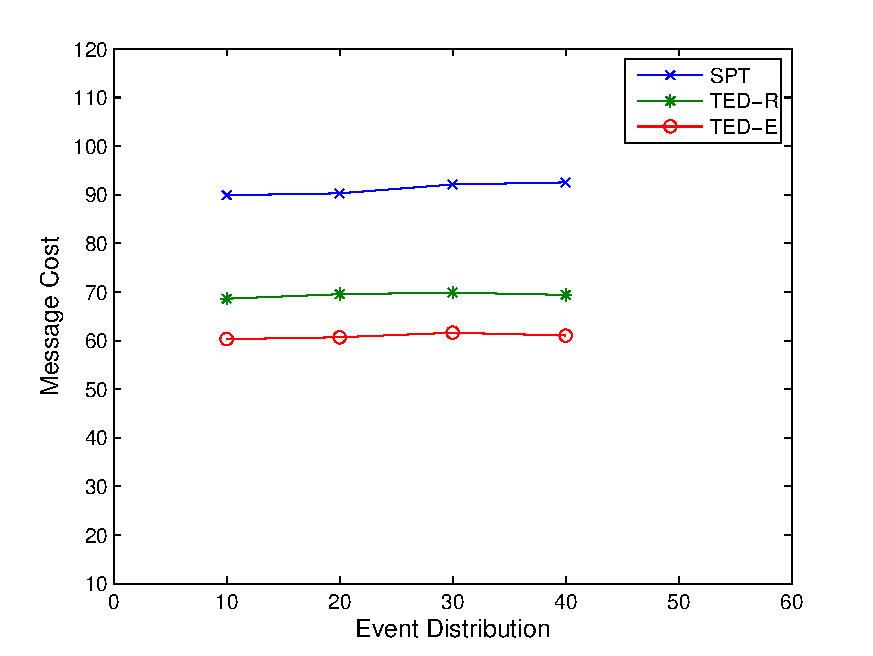
\includegraphics[width=.24\textwidth]{distance-probability80}}
\subfloat[Event probability: 60\%]{\label{fig:sim-distance-probability60}
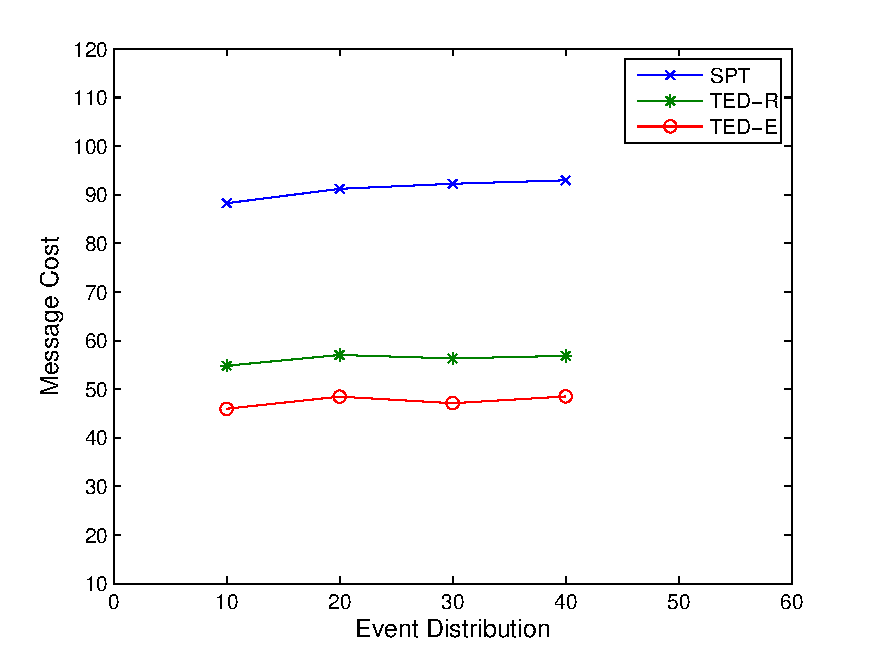
\includegraphics[width=.24\textwidth]{distance-probability60}}
\qquad
\subfloat[Event distance: 20]{\label{fig:sim-probability-distance20}
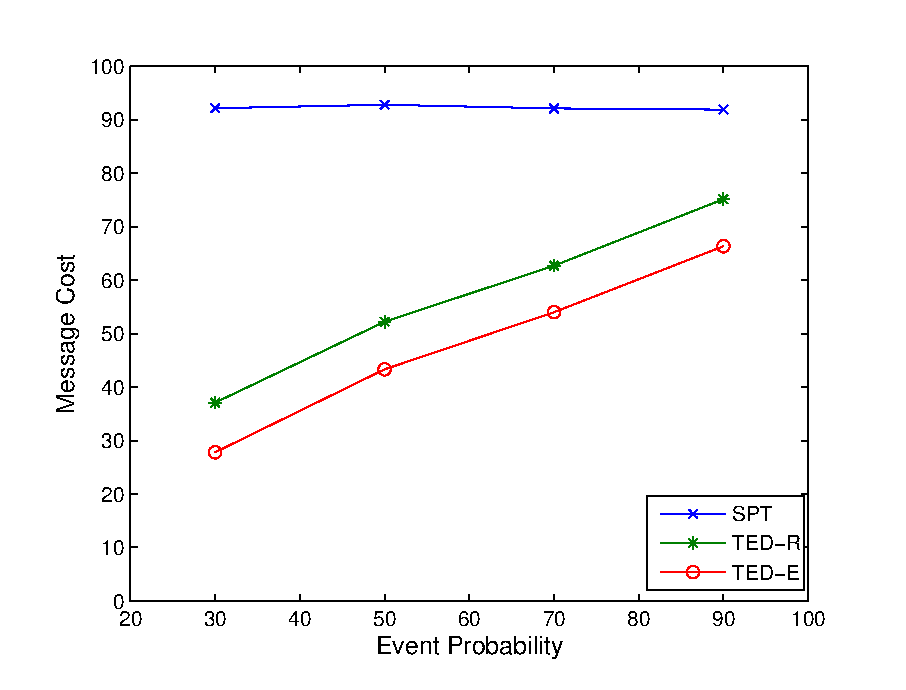
\includegraphics[width=.24\textwidth]{probability-distance20}}
\subfloat[Event distance: 40]{\label{fig:sim-probability-distance40}
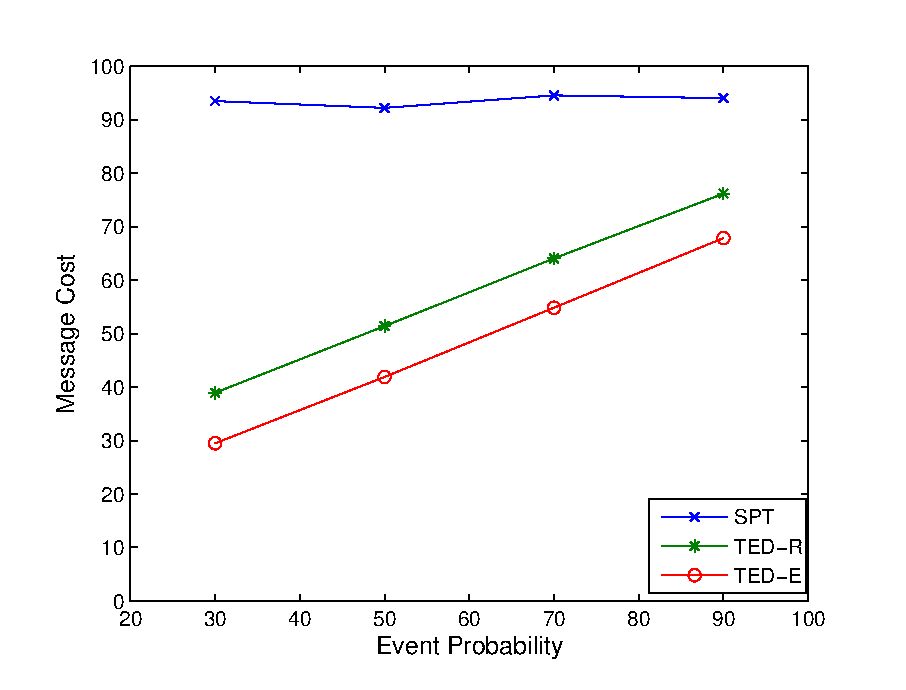
\includegraphics[width=.24\textwidth]{probability-distance40}}
\caption{Simulation results}
\label{fig:sim-all}
\end{figure}

Figure \ref{fig:sim-all} shows all our simulation results. \subref{fig:sim-distance-probability80} and \subref{fig:sim-distance-probability60} show the performance of TED as the event distribution changes. The distribution changes are characterized by the change in the expected distance between the events. We study this type of events because they may be useful to certain applications where you want to detect co-related events that may be far away from each other. We also conducted the simulation based on different event probabilities. TED can outperform SPT by at least 10-20\%. When the probability is lower, TED can further reduce the energy cost.

\subref{fig:sim-probability-distance20} and \subref{fig:sim-probability-distance40}are another set of simulation that shows the relation between cost and event distribution. In general, the energy cost of TED is linearly proportional to the event probability while the energy cost of SPT has little difference in regard to probability changes. This is because TED can efficiently filter a lot of events if their sub-events don't occur so these filtered events don't have to be delivered to the sink

For all the simulations, we can find that the event probability is a major factor that affects the energy saving by TED. This makes TED particular useful in event-based systems where the primitive events occur very often while the composite events are more rare.

\subsection{Experiments}
\label{sec:experiments}
We have implemented TED on MicaZ on top of PSWare. Similar to Section \ref{sec:ceduanalysis}, we implemented a module that does opportunistic data aggregation based on the existing routing protocol provided by TinyOS for comparison.

We compare the performance using the following metrics:
\begin{itemize}
\item Message cost: this is obtained by setting up a counter inside the sensor node. The counter will be written into flash after the experiment so that we can retrieve it.
\item Event detection delay: we measure the time between the subscription is disseminated and the event is notified.
\end{itemize}

In our experiments, we consider the application for WSN-based Structural Health Monitoring (SHM) system. The objective of such system is to detect damages on structures such as buildings and bridges if they occur. Event detection is important in these applications because the SHM sensors will introduce high energy consumption during damage detection. It is therefore more desirable to wake them up only upon the occurrence of certain events \cite{jangshm}.

Figure \ref{fig:testbed} shows our WSN-SHM testbed. In our experiment, we defined a scenario where the sensor nodes will start to collect the data when a certain vibration pattern is detected. The vibration is detected if the one sensor on the top and another one on the bottom of the model read the vibration data that satisfy certain criteria. The event definition is shown in Listing \ref{prog:shm}.
\begin{lstlisting}[caption=Event definition for SHM, label=prog:shm]
Event Vibration {
	data=System.Vibration;
} where {
	data>THRESHOLD1
}
Event CompVibration {
} on {
	Vibration e1 and
	Vibration e2
} where {
	e1.location=='top' &&
	e2.location=='bottom' &&
	e1.data-e2.data>THRESHOLD2
}
\end{lstlisting}

\begin{figure}
\centering
\subfloat[The testbed]{\label{fig:testbed}\figurehalfwidth{CIMG3851.JPG}}
\subfloat[Parameters used in the experiments]{\label{fig:experimentModel}\figurehalfwidth{experimentModel}}
\caption{TED experiment setup}
\label{fig:experimentSetup}
\end{figure}

We manually generate events by hitting the model. Similar to our simulation, we implemented a na\"{i}ve event detection method where the nodes simply use the existing routings provided by TinyOS \cite{nesc} and detect events opportunistically. We implement two modules for both our TED and the opportunistic filtering where only the primitive events are filtered. In order to create multi-hop communication, we adjust the nodes communication range so that they can only communicate with nearby neighbors. For TED, we use tested both the centralized and the distributed versions and for the distributed version. For TED, we have the parameters set as shown in Figure \ref{fig:experimentModel} where \(x\) is the height of the model. The sensor nodes can communicate with other sensor nodes up to 2 floors away. According to the calculation, two fusion points were deployed in the model.

Figure \ref{fig:exp-all} shows all our experimental results. In addition to energy efficiency, we also studied delay. We calculate the delay for TED as the duration between the time that na\"{i}ve approach detects the event and the time that TED detects them. This is because na\"{i}ve approach sends all the detected primitive events directly to the sink and the delay is only introduced by the multi-hop routing latency while both TED have additional delay in detecting the events. The experimental results are expected because TED slightly introduces more delay when doing the fusion points selection. The results on message cost is similar to our simulations.

\begin{figure}
\centering
\subfloat[Message cost]{\label{fig:exp-cost-probability}
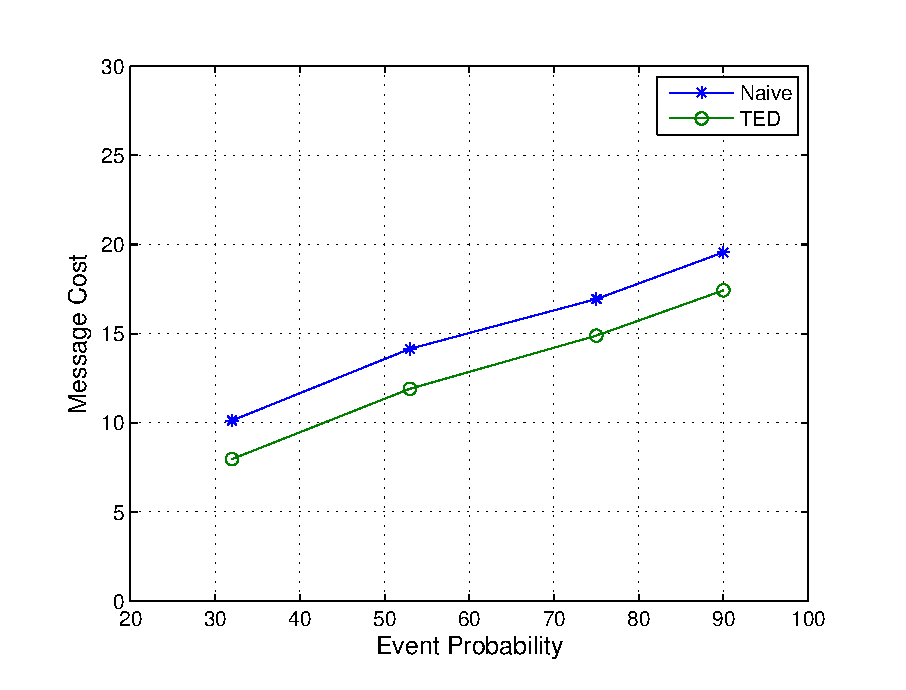
\includegraphics[width=.22\textwidth]{exp-cost}}
\subfloat[Delay]{\label{fig:exp-delay-probability}
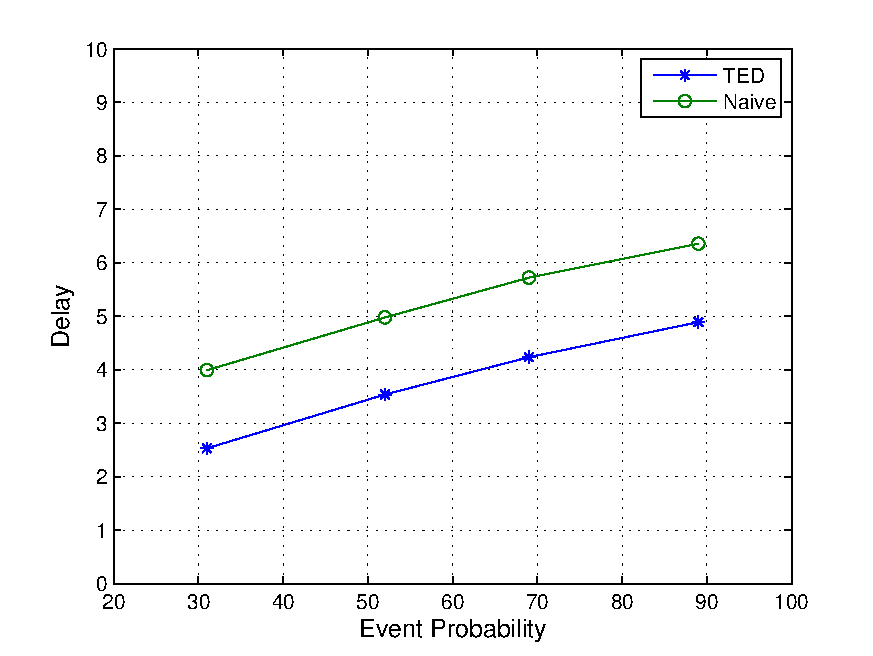
\includegraphics[width=.22\textwidth]{exp-delay}}
\caption{Experimental results}
\label{fig:exp-all}
\end{figure}
